\documentclass[12pt]{article}

\usepackage{amsmath}
\usepackage{amssymb}
\usepackage{amsthm}
\usepackage{centernot}
\usepackage{fullpage}
\usepackage{makecell}
\usepackage{tabularx}
\usepackage[hypcap=false]{caption}
\usepackage[dvipsnames]{xcolor}
\usepackage{tikz,tkz-euclide}
\usetikzlibrary{decorations.pathreplacing,arrows}
\usetikzlibrary{quotes,angles,calc,intersections}
\usepackage{pgfplots}
\pgfplotsset{compat=1.17}

\usepackage{titling}
\usepackage{pdfpages}
\usepackage{color}
\usepackage{hyperref}
\usepackage{enumitem}
\usepackage{multicol}
\usepackage{bm}

\usepackage{common}
\usepackage{linear}

\begin{document}

\title{Signals and Systems}
\author{Brendan Burkhart}
\maketitle

\tableofcontents
\newpage

\section{Introduction}

Signals can be broadly classified into discrete and continuous signals. For example, a continuous signal might be a function of a real variable representing time, or real variables representing a position in space, while a discrete signal is indexed by one or more integer variables. The variable(s) the signal is a function of are the \emph{independent variable(s)} of the signal, the values of the function are the dependent variables. For example, the voltage through a resistor could be the dependent variable of a signal where time is the independent variable.

Signals in the real world are usually continuous signals, but are often discretized for representing in computers and data into discrete signals. A \emph{digital} signal is a discrete signal where the dependent variable(s) have finite precision, which is what signals in a digital representation must be.

The value of a continuous signal $f$ at time $t \in \R$ is commonly denoted by $f(t)$, while a discrete signal $f$ at step $n \in \N$ would be denoted by $f[n]$. That is, parentheses are used for continuous signals, and square brackets for discrete.

Systems are processes, either physical ones like electronics and mechanics, or virtual ones like a software algorithm, that have input and output signals, generating the output signals based on the input signals and any internal state.

\section{Shifting and scaling signals}

Consider a continuous signal $f(t)$. We can shift and scale the amplitude of this signal or we can shift and scale the frequency (or both of course).

Given a signal $f(t)$, $af(t)$ will \emph{scale} the amplitude by a factor of $a$, while $f(t) + b$ will \emph{shift} the amplitude by $b$. Figure \ref{fig:amplitude-scale-shifts} shows a signal $f(t)$ in blue, as well as:
\begin{itemize}
    \item $2f(t)$ in red,
    \item $\frac{1}{2}f(t)$ in green,
    \item and $f(t) + \frac{1}{2}$ in orange.
\end{itemize}

\begin{figure}[ht!]
    \centering
    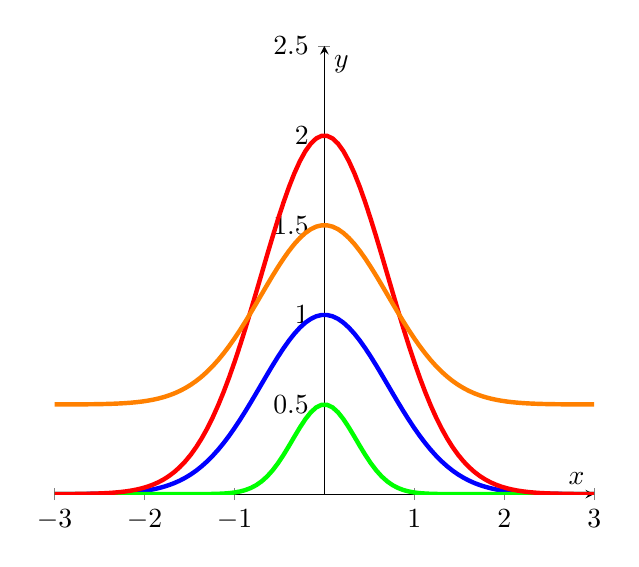
\begin{tikzpicture}[scale=1.0]
        \begin{axis}[
            axis x line=middle,
            axis y line=middle,
            ymin=0,ymax=2.5,ylabel=$y$,
            xmin=-3,xmax=3,xlabel=$x$
            ]

            \addplot[domain=-3:3, blue, ultra thick, samples=100] {e^(-x^2)};
            \addplot[domain=-3:3, green, ultra thick, samples=100] {0.5*e^(-(2*x)^2)};
            \addplot[domain=-3:3, red, ultra thick, samples=100] {2*(e^(-x^2))};
            \addplot[domain=-3:3, orange, ultra thick, samples=100] {e^(-x^2) + 0.5};
        \end{axis}
    \end{tikzpicture}
\caption{Amplitude transformations}
\label{fig:amplitude-scale-shifts}
\end{figure}

Given a signal $f(t)$, $f(at)$ will \emph{scale} the time domain by a factor of $\frac{1}{a}$, while $f(t - b)$ will \emph{shift} the time domain by $b$. Note that the opposite transformation is applied to the signal than is directly applied to the function inputs. Figure \ref{fig:time-scale-shifts} shows a signal $f(t)$ in blue, as well as:
\begin{itemize}
    \item $f(2t)$ in red,
    \item $f(\frac{t}{2})$ in green,
    \item and $f(t - 1)$ in orange.
\end{itemize}

It is important to note the different between scaling and then shifting the time of the signal, versus shifting and then scaling. Figure \ref{fig:time-scale-shifts} shows a signal $f(t)$ in blue, as well as:
\begin{itemize}
    \item $f(2(t-1))$ in red,
    \item $f(2t-1)$ in green,
\end{itemize}

\begin{figure}[ht!]
    \centering
    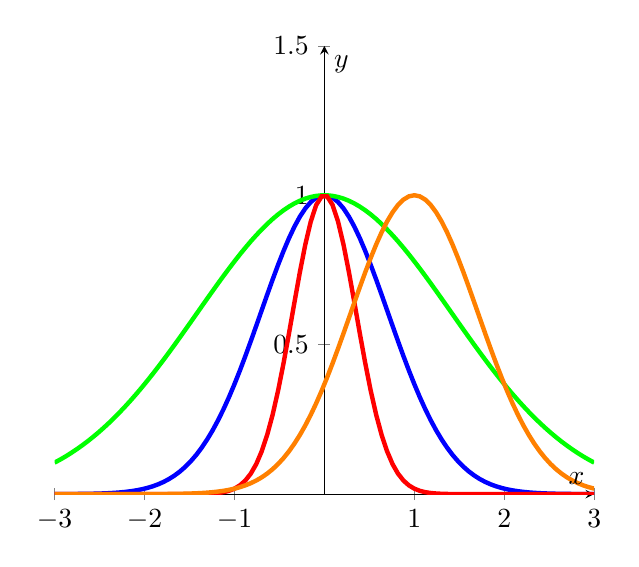
\begin{tikzpicture}[scale=1.0]
        \begin{axis}[
            axis x line=middle,
            axis y line=middle,
            ymin=0,ymax=1.5,ylabel=$y$,
            xmin=-3,xmax=3,xlabel=$x$
            ]

            \addplot[domain=-3:3, blue, ultra thick, samples=100] {e^(-x^2)};
            \addplot[domain=-3:3, green, ultra thick, samples=100] {e^(-(x/2)^2)};
            \addplot[domain=-3:3, red, ultra thick, samples=100] {(e^(-(2*x)^2))};
            \addplot[domain=-3:3, orange, ultra thick, samples=100] {e^(-(x-1)^2)};
        \end{axis}
    \end{tikzpicture}
\caption{Time transformations}
\label{fig:time-scale-shifts}
\end{figure}

\begin{figure}[ht!]
    \centering
    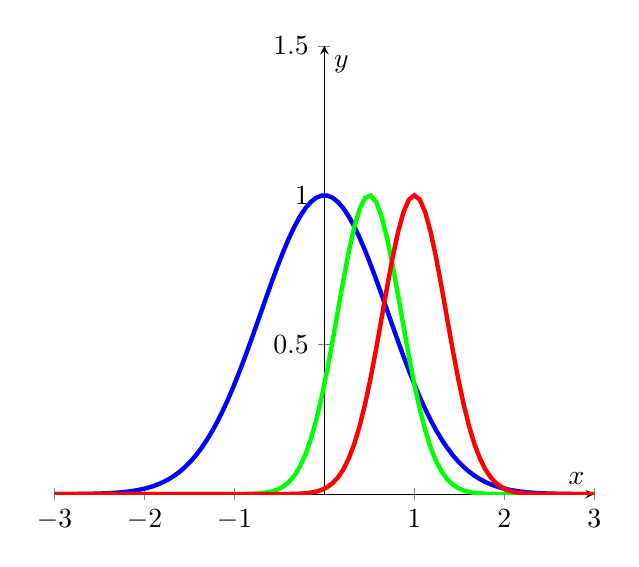
\begin{tikzpicture}[scale=1.0]
        \begin{axis}[
            axis x line=middle,
            axis y line=middle,
            ymin=0,ymax=1.5,ylabel=$y$,
            xmin=-3,xmax=3,xlabel=$x$
            ]

            \addplot[domain=-3:3, blue, ultra thick, samples=100] {e^(-x^2)};
            \addplot[domain=-3:3, green, ultra thick, samples=100] {e^(-(2*x-1)^2)};
            \addplot[domain=-3:3, red, ultra thick, samples=100] {e^(-(2*(x-1))^2};
        \end{axis}
    \end{tikzpicture}
\caption{Time transformations 2}
\label{fig:time-scale-shifts-2}
\end{figure}

\section{Common signals}

Two of the most common discrete signals are the unit impulse signal, and the unit step signal. The unit impulse is also known as the delta function and so is commonly denoted by $\delta[n]$, and is defined by
\[\delta[n] =
\begin{dcases}
    1, & n = 1 \\
    0, & n \neq 0
\end{dcases}.\] The unit step signal $u[n]$ is defined by
\[u[n] = \sum_{m=-\infty}^{n}\delta[m].\] Note that $\delta[n] = u[n] - u[n-1]$.

\begin{figure}[ht!]
    \centering
    \begin{tikzpicture}[scale=1.0]
        \begin{axis}[
            axis x line=middle,
            axis y line=middle,
            ymin=0,ymax=1.5,ylabel=$y$,
            xmin=-3,xmax=3,xlabel=$x$
            ]

            \addplot+[const plot, no marks, ultra thick] coordinates {(-3,0) (0,0) (0,1) (0,0) (3,0)};
        \end{axis}
    \end{tikzpicture}
\caption{Unit impulse signal}
\label{fig:unit-impulse}
\end{figure}

\begin{figure}[ht!]
    \centering
    \begin{tikzpicture}[scale=1.0]
        \begin{axis}[
            axis x line=middle,
            axis y line=middle,
            ymin=0,ymax=1.5,ylabel=$y$,
            xmin=-3,xmax=3,xlabel=$x$
            ]

            \addplot+[const plot, no marks, ultra thick] coordinates {(-3,0) (0,0) (0,1) (3,1)};
        \end{axis}
    \end{tikzpicture}
\caption{Unit step signal}
\label{fig:unit-step}
\end{figure}

\end{document}
